\paragraph{Échéancier :}
Utilisation d'un échancier suivant le modèle du diagramme de Gantt réalisé à l'aide de MS Project. Il est divisé en trois captures d'écran à des fins pratiques.

\begin{figure}[ht!]
    \centering
    \caption{Échéancier partie 1}
    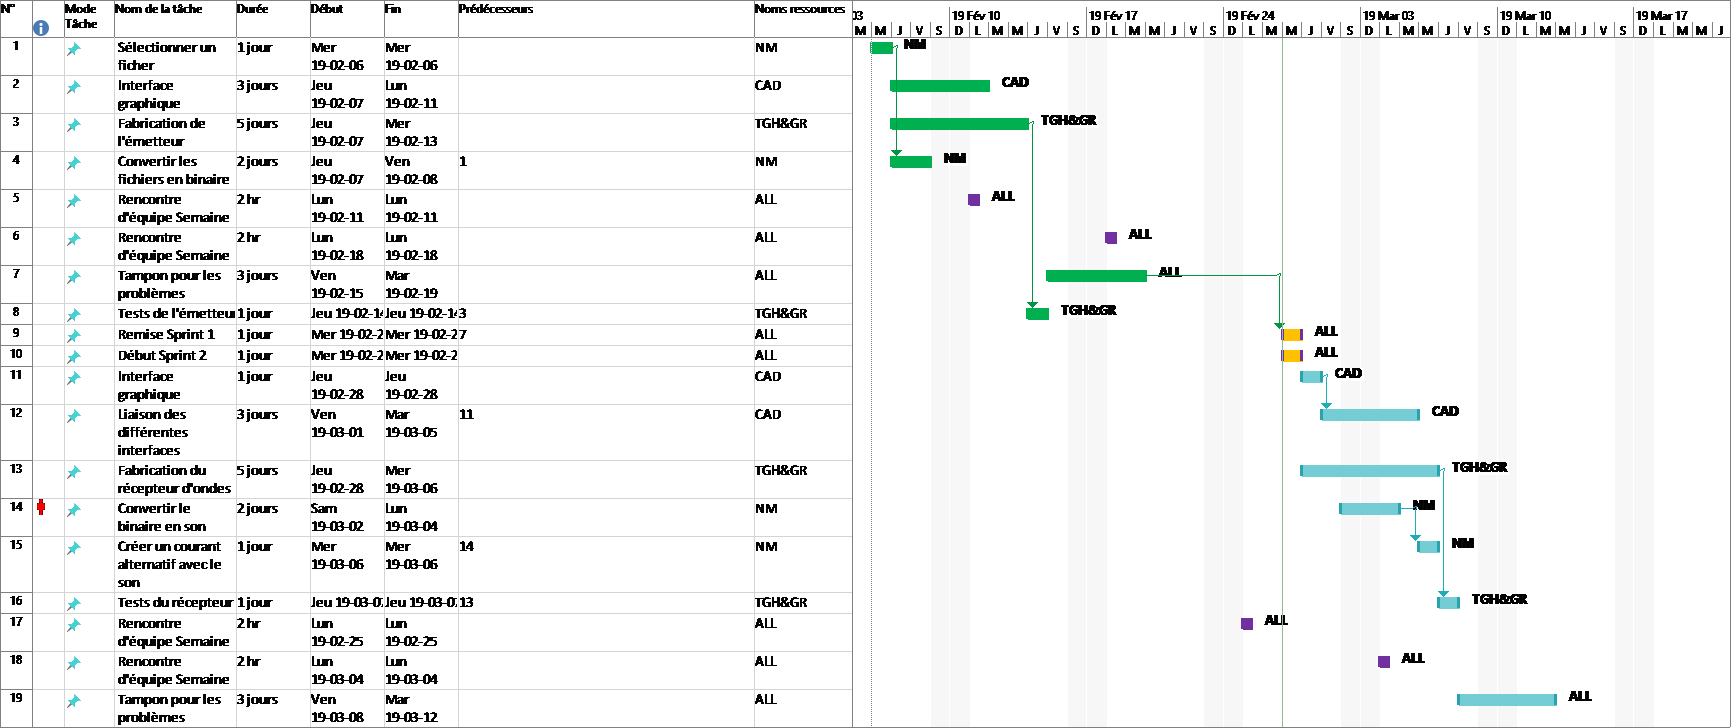
\includegraphics[width=0.8\linewidth]{images/echeancier/echeancier_Sprint_2_part1.png}
\end{figure}

\begin{figure}[ht!]
    \centering
    \caption{Échéancier partie 2}
    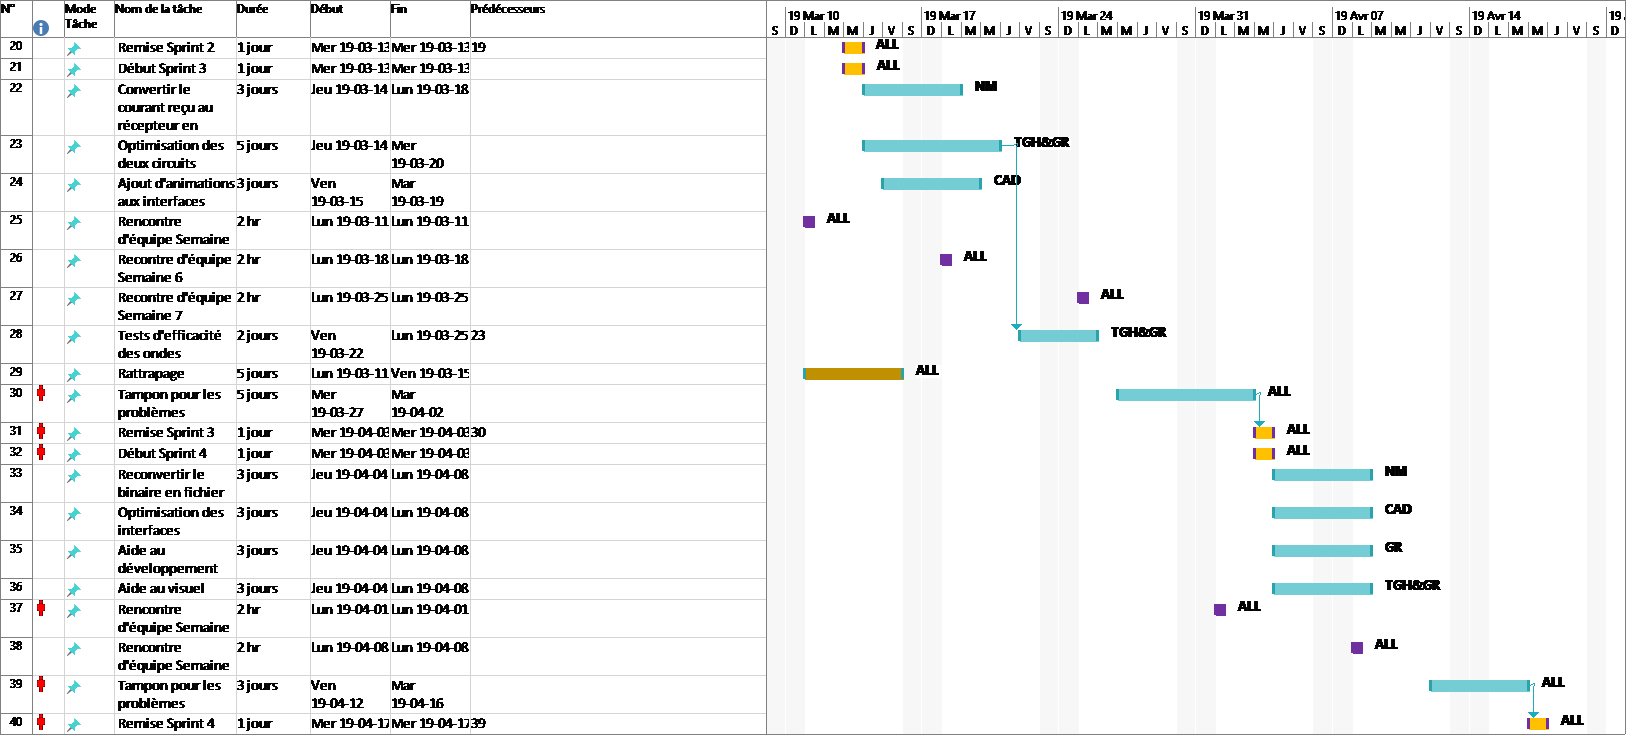
\includegraphics[width=0.8\linewidth]{images/echeancier/echeancier_Sprint_2_part2.png}
\end{figure}

\begin{figure}[ht!]
    \centering
    \caption{Échéancier partie 3}
    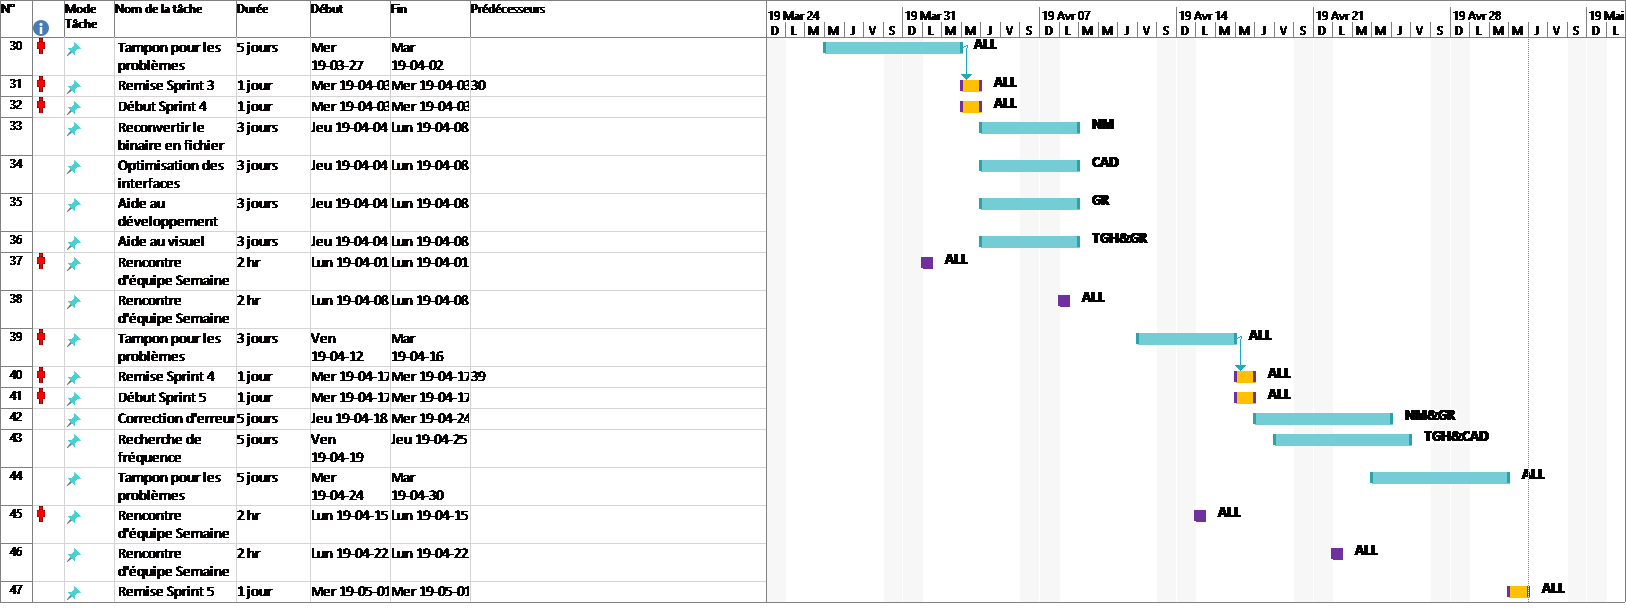
\includegraphics[width=0.8\linewidth]{images/echeancier/echeancier_Sprint_2_part3.png}
\end{figure}